%%******************************************************************************
%%
%% introduction.tex
%%
%%******************************************************************************
%%
%% Title......: Introduction
%%
%% Author.....: GSCAR-DFKI
%%
%% Started....: Nov 2013
%%
%% Emails.....: alcantara@poli.ufrj.br elael@poli.ufrj renan028@gmail.com
%%
%% Address....: Universidade Federal do Rio de Janeiro
%%              Caixa Postal 68.504, CEP: 21.945-970
%%              Rio de Janeiro, RJ - Brasil.
%%
%%******************************************************************************


%%******************************************************************************
%% SECTION - Eletronica
%%******************************************************************************

\section{Proposta 2 – PC Embarcado e base com Roteador}

\subsection{Arquitetura da Eletrônica Proposta 2}
A solução com um PC embarcado, acoplado à estrutura do Lifting Beam, é
considerada uma solução intermediária em relação ao custo e é uma solução que
mais se aproxima ao produto final. Esta solução é menos suscetível a falhas
elétricas e de gerenciamento de dispositivos, quando comparada com a solução da
placa com microcontrolador. Além disso, o tempo de execução gasto para programação de microcontrolador e fabricação da placa justifica a aquisição de um PC104. Na figura~\ref{pc104}, podemos observar o diagrama de interfaces desta solução.

\begin{figure}[H]
    \centering
    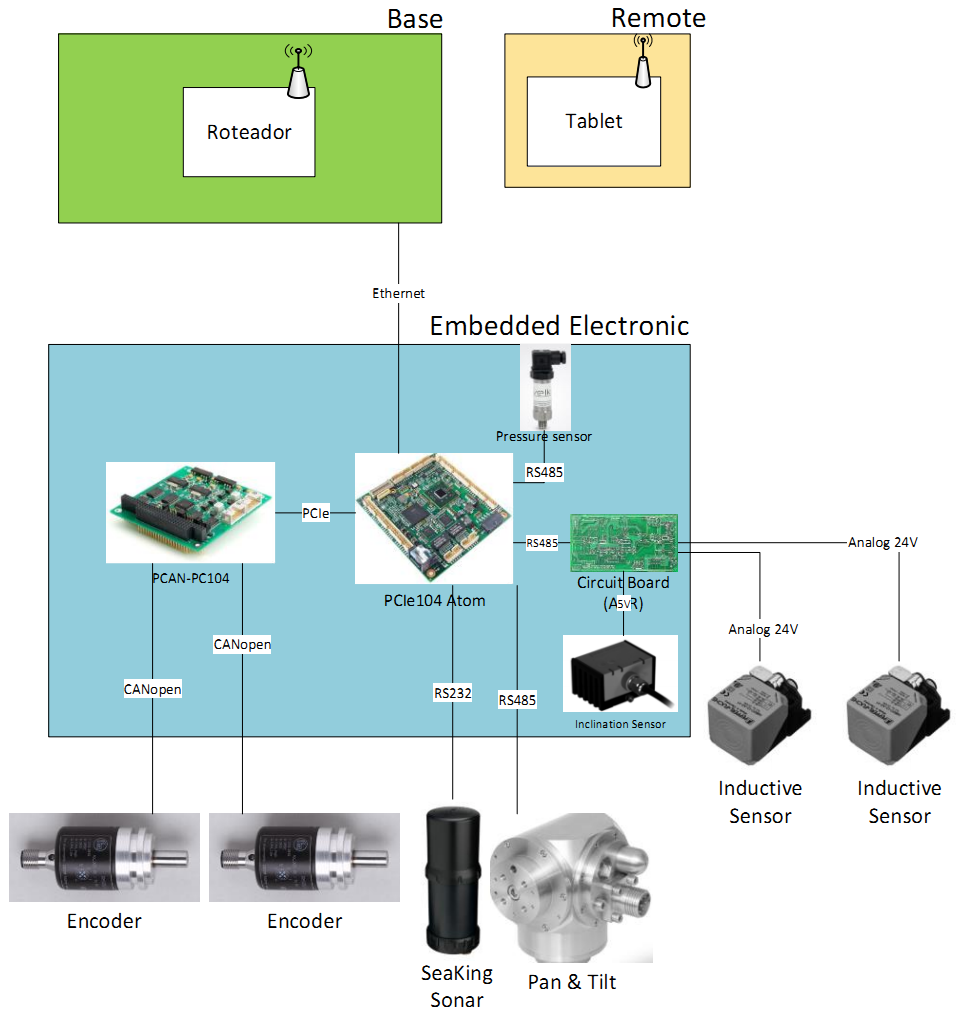
\includegraphics[width=1\columnwidth]{figs/eletronica/4.png}
    \caption{Diagrama de Comunicações - PC104}
    \label{pc104}
\end{figure} 
 
Assim como a solução 1, deverá ser construída uma estrutura mecânica à prova d’água.

\subsection{Arquitetura de Software Proposta 2}

Para esta proposta o processamento dos dados aquisitados pelos sensores será
processado na própria eletrônica embarcada e, em seguida,
 serão enviados para o tablet, podendo ser roteado por um computador em terra ou
 diretamente por um roteador, figura \ref{fig:FL:2}.
 
 \afterpage{
\begin{landscape}
 \begin{figure}
  \centering
  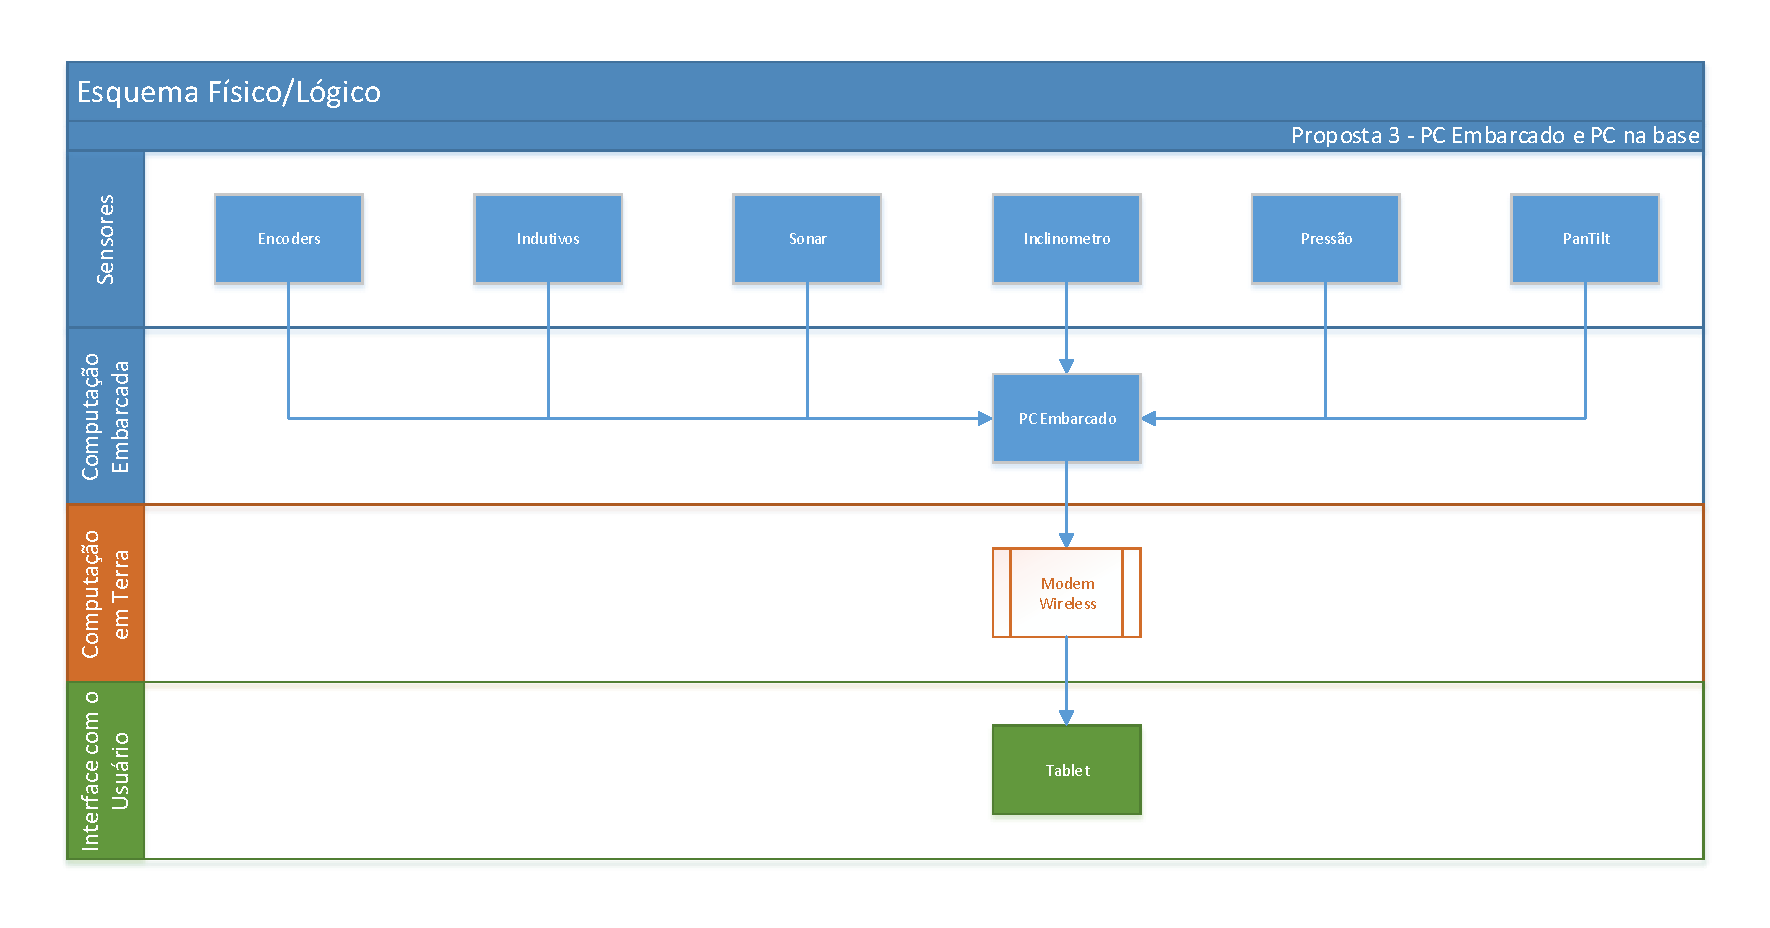
\includegraphics[width=1\linewidth,keepaspectratio]{figs/software/LogicoFisico/EsqLogicoFisico2n.pdf}
  \caption{Relação entre os componentes físicos e as divisões lógicas da
  proposta 2.}
  \label{fig:FL:2}
 \end{figure}
\end{landscape}
}

Cada sensor deverá possuir, novamente, um driver para a interface entre o
equipamento físico e camada de software, isto é, os encoders, inclinômetro, os
sensores indutivos e o sensor de pressão possuirão drivers dedicados para a
leitura de dados, feita através de uma conexão Ethernet para a placa que
interconecta os sensores. O sonar e o módulo PanTilt também possuirão drivers
próprios para a aquisição de dados e controle.

Todos os componentes principais estão localizados no computador embarcado, o
inverso do que ocorre na proposta 1, sendo assim a figura \ref{fig:FL:1} uma
imagem dos compontes embarcados.O componente de software responsável pela
monitoração irá processar e conformar os dados provenientes dos sensores
utilizados para o monitoramento das operações de inserção e remoção (encoders,
inclinômetro, sensores indutivos e sensor de pressão). Os dados provenientes do
sonar devem ser integrados com a posição do elemento PanTilt, no componente
Sonar-PanTilt, para que sejam consistentes e completos. O módulo de Reconstrução
3D é responsável, então, por  traduzir os dados processados pelo componente
anterior em uma visualização inteligível para o ser humano. Um componente de
segurança também é adicionado para monitorar a correta utiliza\-ção do sonar
(apenas embaixo d’água), conferindo uma maior robustez ao sistema.

Após o processamento dos dados, será estabelecida uma conexão wi-fi com o tablet
por meio de um computador em terra ou
 apenas por meio de um roteador.
 
Os componentes da interface homem máquina permanecem inalterados em relação à
proposta anterior.